\documentclass[12pt]{report}
\usepackage{hyperref}
\hypersetup{
	colorlinks=true,
	linkcolor=blue,
	filecolor=magenta,      
	urlcolor=cyan,
	pdftitle={Overleaf Example},
	pdfpagemode=FullScreen,
}
\usepackage{graphicx}

\title{AI code generation report}
\author{Roblox prime numbers:\\\small{Oleh Basystyi}\\\small{Anna Stasyshyn}
\\\small{Artur Rudish}\\\small{Anton Valihurskyi}\\\small{Maksym Zhuk}}
\date{April 2024}
\begin{document}
	\maketitle	
	\renewcommand{\thesection}{\arabic{section}}
	\section{Introduction}
	In this little survey out team have researched AI's capability to solve CodeWars tasks of different difficulty (primarily 7, 6, 5, 4 kyu) and different CodeWars cagtegories:
	\begin{itemize}
		\itemsep0em 
		\item Algorithms
		\item Strings
		\item Arrays
		\item Mathematics
		\item Linear Algebra
		\item Dynamic Programming
		\item Data Structures
	\end{itemize}
	As AIs we used \textit{GPT-3.5, GPT-4, Claude} and \textit{Gemini} and compared their performance on same tasks. Also we researched two ways of writting prompts to solve problems like this: templated and manual that must be used in different cases
	
	\pagebreak
	\section{Experimenting}
	To carefully carry out experiments we have set up \href{https://docs.google.com/spreadsheets/d/1qXPyAJsOOpmtxIoGqObwG5mTaLU3IWO0SQRGbjZPhEc/edit#gid=0}{google sheets table} to log data about AI performance on solving particular tasks. In total we analyzed 18 problems and gained that kind of data:
	
	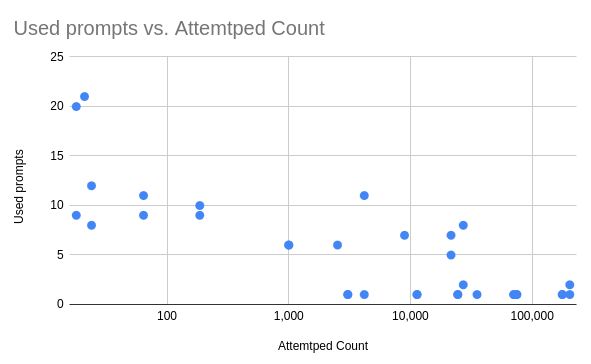
\includegraphics[width=\textwidth]{used_prompts_attempted_relation.png}
	
	It shows the relation between number of perople that attempted to solve a particular problem and number of prompts that we have used to make AI solve it. As can be seen from char the general rule is that tasks attempted by smaller amount of perople was more difficult to solve by AI. And actually we can see a breakpoint around region of 1000 attempts. Due to this we have used different techniques to get problem solution from AI
	
\end{document}